\chapter{ORGANIZAÇÃO DIDÁTICO PEDAGÓGICA}
\label{chap:matriz}

O curso Superior de Engenharia Eletrônica do Câmpus Toledo da UTFPR  é estruturado de acordo com: a Lei nº 9.131, de 24 de novembro de 1995 \cite{Lei:9131:1995}; a Lei nº 9.394, de 20 de dezembro de 1996 \cite{Lei:9394:1996}; a Lei nº 11.184, de 7 de outubro de 2005 \cite{Lei:11.184:2005}; o Estatuto e Regimento Geral da UTFPR \cite{estatutoutfpr}; as Diretrizes Curriculares Nacionais do Curso de Graduação em Engenharia \cite{dcneng}; a Resolução n\textordmasculine{} 142/2022 – COGEP/UTFPR, de 25 de fevereiro de 2022 \cite{cogep142}; e às demais diretrizes e regulamentos internos aplicáveis. A concepção de ensino e aprendizagem do curso, a matriz curricular, os procedimentos de avaliação e os instrumentos de apoio expressos no Projeto Pedagógico de Curso (PPC), são construídos coletivamente e submetidos ao Conselho de Graduação e Educação Profissional (COGEP) para aprovação, em modelo e prazo estabelecido.

Segundo o PPI:

\begin{citacao}
	``A  UTFPR  deve  contribuir  para  o  avanço  conceitual  da educação profissional e tecnológica, tomando como princípio a formação integral do homem,  em  bases  científicas  e  ético-políticas,  entendendo  que  o  exercício  das atividades humanas não se restringe ao caráter produtivo, mas compreende todas as dimensões: social, política, cultural e ambiental'' \cite{ppiutfpr}.
\end{citacao}

Dessa forma, a estrutura curricular do Curso de Engenharia Eletrônica da UTFPR – Campus Toledo possui bases na demanda do mercado regional (veja a \autoref{sec:const}), demanda essa tanto de qualificação profissional, como de características socioeconômicas. Para dar atendimento à demanda do mercado de um profissional com um perfil diferenciado, não só em tecnologia, mas também voltado para o desenvolvimento social e sustentabilidade, a organização do Curso de Engenharia Eletrônica apresenta bases científicas e de gestão de nível superior dimensionada e direcionada às terminalidades da formação do engenheiro.

A organização didático pedagógica deste PPC promove as políticas de ensino e de graduação, previstas nos documentos institucionais norteadores PDI \cite{pdiutfpr} e PPI \cite{ppiutfpr}. As políticas de ensino são as elencadas na seção ``3.3 POLÍTICAS DE ENSINO'' do PDI:

\begin{itemize}
	\item Articulação entre a teoria e a prática;
	\item Desenvolvimento de competências profissionais;
	\item Flexibilidade curricular;
	\item Mobilidade acadêmica;
	\item Articulação entre ensino, pesquisa e extensão.
\end{itemize}

Da mesma forma, as políticas de graduação são elencadas na seção ``3.4 POLÍTICAS DE GRADUAÇÃO'' do PDI:

\begin{itemize}
	\item Flexibilidade curricular;
	\item Articulação com a sociedade;
	\item Mobilidade acadêmica;
	\item Sustentabilidade;
	\item Interculturalidade;
	\item Inovação curricular e metodológica;
	\item Internacionalização.
\end{itemize}

O Curso de Engenharia Eletrônica promove a aprendizagem de conhecimentos estruturados vinculados ao desenvolvimento de competências, em uma dinâmica que enfatiza a prática profissional sem excluir as dimensões sociais e ambientais da qual faz parte. As disciplinas, não mais isoladas, são promotoras do saber, saber fazer e saber ser, se responsabilizando pelo currículo vivo formador de profissionais aptos a mobilizar, integrar e aplicar adequadamente esses conhecimentos. A metodologia do curso envolve processos de participação do estudante que permite a constante construção do conhecimento.

Os conceitos são apresentados a partir dos conhecimentos expostos em livros didáticos, artigos científicos, situações reais e outros materiais bibliográficos pertinentes, conduzidos pela experiência dos docentes. Também são incentivados projetos que permitam a análise reflexiva e o aprendizado da prática profissional pelo discente. Procura-se continuamente estabelecer a interdisciplinaridade relacionando os conteúdos das diversas disciplinas que compõem o curso.

A estrutura apresentada, propõe a intencionalidade em trabalhar habilidades e atitudes do futuro engenheiro. O corpo docente, com sua experiência adquirida, permitirá momentos de aprendizagem relacionados ao desenvolvimento dessas habilidades e atitudes através de um projeto de currículo para esse fim.

Neste contexto, esse projeto de estrutura curricular é apresentado em detalhes nas seções posteriores, bem como sua relação com as políticas de ensino e de graduação indicadas no início desta seção.


\section{ORGANIZAÇÃO CURRICULAR}

A matriz curricular do curso de Engenharia Eletrônica da UTFPR é estruturada em dez semestres sob o regime de matrícula por disciplina com entrada anual de 88 acadêmicos. Sua carga horária totaliza \the\value{horasT} h de atividades com conteúdo de natureza profissionalizante, científica, humanística, extensionista e cultural.

A organização da matriz curricular do curso contempla os objetivos de instigar o interesse pela ciência e tecnologia e, ao mesmo tempo, fornece um sólido embasamento para o conteúdo profissionalizante. Isto é alcançado apresentando disciplinas profissionalizantes o mais cedo possível, ao mesmo tempo que o aluno tem uma prévia do que será ministrado adiante no curso através da disciplina de Introdução à Engenharia. A maioria das disciplinas possui carga horária em laboratório, com experimentos realizados nas áreas de física, química e eletrônica desde o primeiro semestre. As disciplinas da área de formação profissionalizante estão presentes a partir do terceiro semestre e são desenvolvidas em sua maior parte em laboratório. Especificamente, os conteúdos de computação são apresentados desde o primeiro semestre, enquanto os conteúdos de engenharia elétrica e eletrônica são apresentados desde o terceiro. Além disso, a sequência de pré-requisitos das disciplinas permite a inclusão de atividades interdisciplinares desde o início do curso.

%As atividades acadêmicas presenciais são divididas em Atividades Teóricas (AT) e Atividades Práticas (AP). As ATs consistem na apresentação de conteúdos teóricos em sala de aula. Já as APs têm vistas ao desenvolvimento prático dos conteúdos, consistindo de experimentos, atividades de laboratório, ou visitas técnicas. 

As atividades acadêmicas são divididas em atividades teóricas (AT) e práticas (AP), conforme Art. 20 das Diretrizes Curriculares dos Cursos de Graduação Regulares da UTFPR \cite{cogep142}. As ATs correspondem às atividades, de caráter presencial ou não, utilizadas para o desenvolvimento e compreensão de conceitos e de teorias. Já as AP têm vistas às atividades, de caráter presencial ou não, utilizadas para o desenvolvimento prático de conteúdos, tais como: atividades de laboratório, desenvolvimento de projetos, estudos de caso, visitas técnicas, levantamentos em campo, produção de textos, dentre outras.

%O Art. 24 em seu parágrafo 1\textordmasculine{} considera que os projetos pedagógicos dos cursos da UTFPR devem dar ênfase a AP. Para cursos de Engenharia, a carga horária de AP deve ser coerente com a formação pretendida. Objetiva-se, com isto, formar um profissional diferenciado, apto a lidar com problemas de ordem prática e pronto para lidar com as necessidades imediatas do mercado de trabalho.

Algumas unidades curriculares também possuem parte da carga horária  em atividades não-presenciais (ANP), que correspondem a processos de ensino e aprendizagem desenvolvidos para além dos tempos e espaços da sala de aula. São mediadas por tecnologias digitais de informação e comunicação, desenvolvidas numa relação dialógica entre docentes e estudantes.

\nomenclature[A]{AT}{Atividades Teóricas}
\nomenclature[A]{AP}{Atividades Práticas}
\nomenclature[A]{ANP}{Atividades não-Presenciais} 

O curso de Engenharia Eletrônica dá ênfase as APs. Objetiva-se, com isto, formar um profissional diferenciado, apto a lidar com problemas de ordem prática e pronto para lidar com as necessidades imediatas do mercado de trabalho.



%A Construção curricular deve responder diretamente aos objetivos formativos. Considerando as metas educacionais para formação profissional percebe-se que para alcança-las os projetos de ensino superior precisam propor mudanças significativas e inovadoras em suas organizações curriculares.

%Assim, é imperativo a construção de currículos inovadores e estrategicamente orientados à aprendizagem significativa, ao desenvolvimento integrado e sustentável, às necessidades, aspirações e expectativas dos alunos e à transformação da realidade em que vivem.

%No início da apresentação da organização curricular deve conter a proposta que fundamenta o curso, pois, são os fundamentos teórico metodológicos que sustentam as decisões sobre a escolha entre uma ou outra matriz curricular. A organização curricular do curso deve apresentar as unidades curriculares agrupadas por áreas de conhecimento, número de períodos, organização de temas transversais, integração horizontal e vertical. Incluir aqui como será desenvolvido no curso o ciclo de humanidades (art. 25 e 26 da Resolução COGEP 90/2018). Descrever se, como e quanto serão utilizados de momentos de aprendizado não presenciais ao longo do curso


\section{MATRIZ CURRICULAR}
\label{sec:matriz}

A matriz curricular do Curso de Engenharia Eletrônica é construída em consonância com os objetivos do curso e da Instituição, atendendo ao perfil do egresso (ver \autoref{sec:perf}), após as discussões dos integrantes do NDE.

Os conteúdos trabalhados devem ter significado aos estudantes, possibilitando uma aprendizagem consistente e significativa. Entende-se que os conhecimentos técnicos não podem estar separados da formação geral e humanística. Os eixos norteadores, destacados, são considerados prioritários e serão desenvolvidos durante toda a trajetória do curso, quais sejam, como Meio ambiente, Ética e Cidadania, Relações Étnico-Raciais, Direitos Humanos, a construção de valores de solidariedade, inclusão, cooperação e respeito à Diversidade.

A partir desta perspectiva, a estruturação curricular do curso seguindo as diretrizes curriculares para os cursos de Engenharia \cite{dcneng}, é embasada em três Núcleos de Conteúdos, com a necessária interligação entre si:

\begin{enumerate}
	\item 	Núcleo de Conteúdos Básicos;
	\item 	Núcleo Conteúdos Profissionalizantes;
	\item 	Núcleo Conteúdos Profissionalizantes Específicos.
\end{enumerate}

Quanto a extensão, os discentes do Curso podem desenvolver em conjunto com a Universidade:

\begin{itemize}
	\item 	Projetos de Educação e Inclusão Social;
	\item	Ações para Desenvolvimento Econômico e Responsabilidade Social;
	\item	Atividades de Valorização da diversidade, do meio ambiente, da memória cultural, da produção artística e de patrimônio cultural;
	\item	Projetos de Educação Ambiental e de Desenvolvimento Nacional Sustentável.
\end{itemize}

% Retirado do PPC de campo mourão
A estrutura curricular tem como base a demanda do mercado regional e nacional, sendo norteada pela qualificação profissional e ao atendimento das necessidades socioeconômicas. Para dar atendimento à demanda do mercado por profissionais com um perfil diferenciado, não só em tecnologias emergentes, como também voltado para o desenvolvimento social, a organização do Curso de Bacharelado em Engenharia Eletrônica apresenta bases científicas e de gestão de nível superior dimensionada e direcionada às terminalidades da formação do engenheiro. %Estruturada em dez semestres sob o regime de matrícula por unidade curricular, sua carga horária totaliza \the\value{horasT} h de atividades com conteúdo de natureza profissionalizante, científica, humanística e cultural.

%A organização da matriz curricular do curso contempla os objetivos de instigar o interesse pela ciência e tecnologia e, ao mesmo tempo fornecer um sólido embasamento para o conteúdo profissionalizante. Isto é alcançado apresentando disciplinas profissionalizantes o mais cedo possível, ao mesmo tempo em que o aluno tem uma prévia do que será ministrado adiante no curso através da disciplina de Introdução à Engenharia. A maioria das disciplinas possui carga horária em laboratório, com experimentos realizados nas áreas de física, química e eletrônica desde o primeiro semestre. As disciplinas da área de formação profissionalizante estão presentes em quase todos os semestres e são desenvolvidas em sua maior parte em laboratório. Além disso, os conteúdos de engenharia elétrica e eletrônica são apresentados desde o primeiro semestre, buscando a motivação do discente desde o início de sua jornada acadêmica.

%As atividades acadêmicas são divididas em atividades teóricas (AT) e práticas (AP), conforme Art. 20 das Diretrizes Curriculares dos Cursos de Graduação Regulares da UTFPR \cite{cogep142}. As ATs correspondem às atividades, de caráter presencial ou não, utilizadas para o desenvolvimento e compreensão de conceitos e de teorias. Já as AP têm vistas às atividades, de caráter presencial ou não, utilizadas para o desenvolvimento prático de conteúdos, tais como: atividades de laboratório, desenvolvimento de projetos, estudos de caso, visitas técnicas, levantamentos em campo, produção de textos, dentre outras.

%O Art. 24 em seu parágrafo 1\textordmasculine{} considera que os projetos pedagógicos dos cursos da UTFPR devem dar ênfase a AP. Para cursos de Engenharia, a carga horária de AP deve ser coerente com a formação pretendida. Objetiva-se, com isto, formar um profissional diferenciado, apto a lidar com problemas de ordem prática e pronto para lidar com as necessidades imediatas do mercado de trabalho.

%Ainda, o curso desenvolve as ações de: (i) popularização científica e tecnológica; (ii) disseminação tecnológica em escolas do ensino médio e fundamental; (iii) ações para integração com o mundo do trabalho e (iv) projetos de educação ambiental e de desenvolvimento regional sustentável.
%% Fim da cópia

O \autoref{qua:matriz} apresenta a matriz curricular do curso de Engenharia Eletrônica do campus Toledo da UTFPR. \pdfmarkupcomment{As unidades curriculares são codificadas por cores, sendo verde claro: obrigatórias do ciclo de humanidades; verde escuro: optativas do ciclo de humanidades; cinza: optativas específicas; e amarelo: demais unidades curriculares}{Verificar como fica a codificação das cores, até o momento não existe uma orientação.} %As seções \ref{sub:reg} à \ref{sub:extch} resumem as informações do referido quadro.

As unidades curriculares do curso, apresentadas na matriz anterior (\autoref{qua:matriz}), apresentam em sua constituição carga horária teórica e prática, com codificação em cada unidade curricular, conforme apresentado na \autoref{fig:legenda}. Portanto, diversas disciplinas promovem a política de ensino ``Articulação entre teoria e prática''.

\begin{figure}[hbt!]
	\centering
	\caption{Codificação das unidades curriculares da Matriz}
	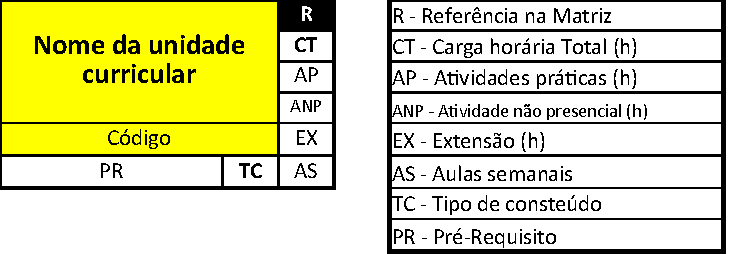
\includegraphics[width=0.6\textwidth]{Caps/Figs/Matriz_final_v2_leg.pdf}
	\fonte{\utf}
	\label{fig:legenda}
\end{figure}

\newgeometry{textwidth=200mm,textheight=290mm}
\begin{landscape}
	\begin{quadro}
		\centering
		\caption{Matriz do Curso de Engenharia Eletrônica}
		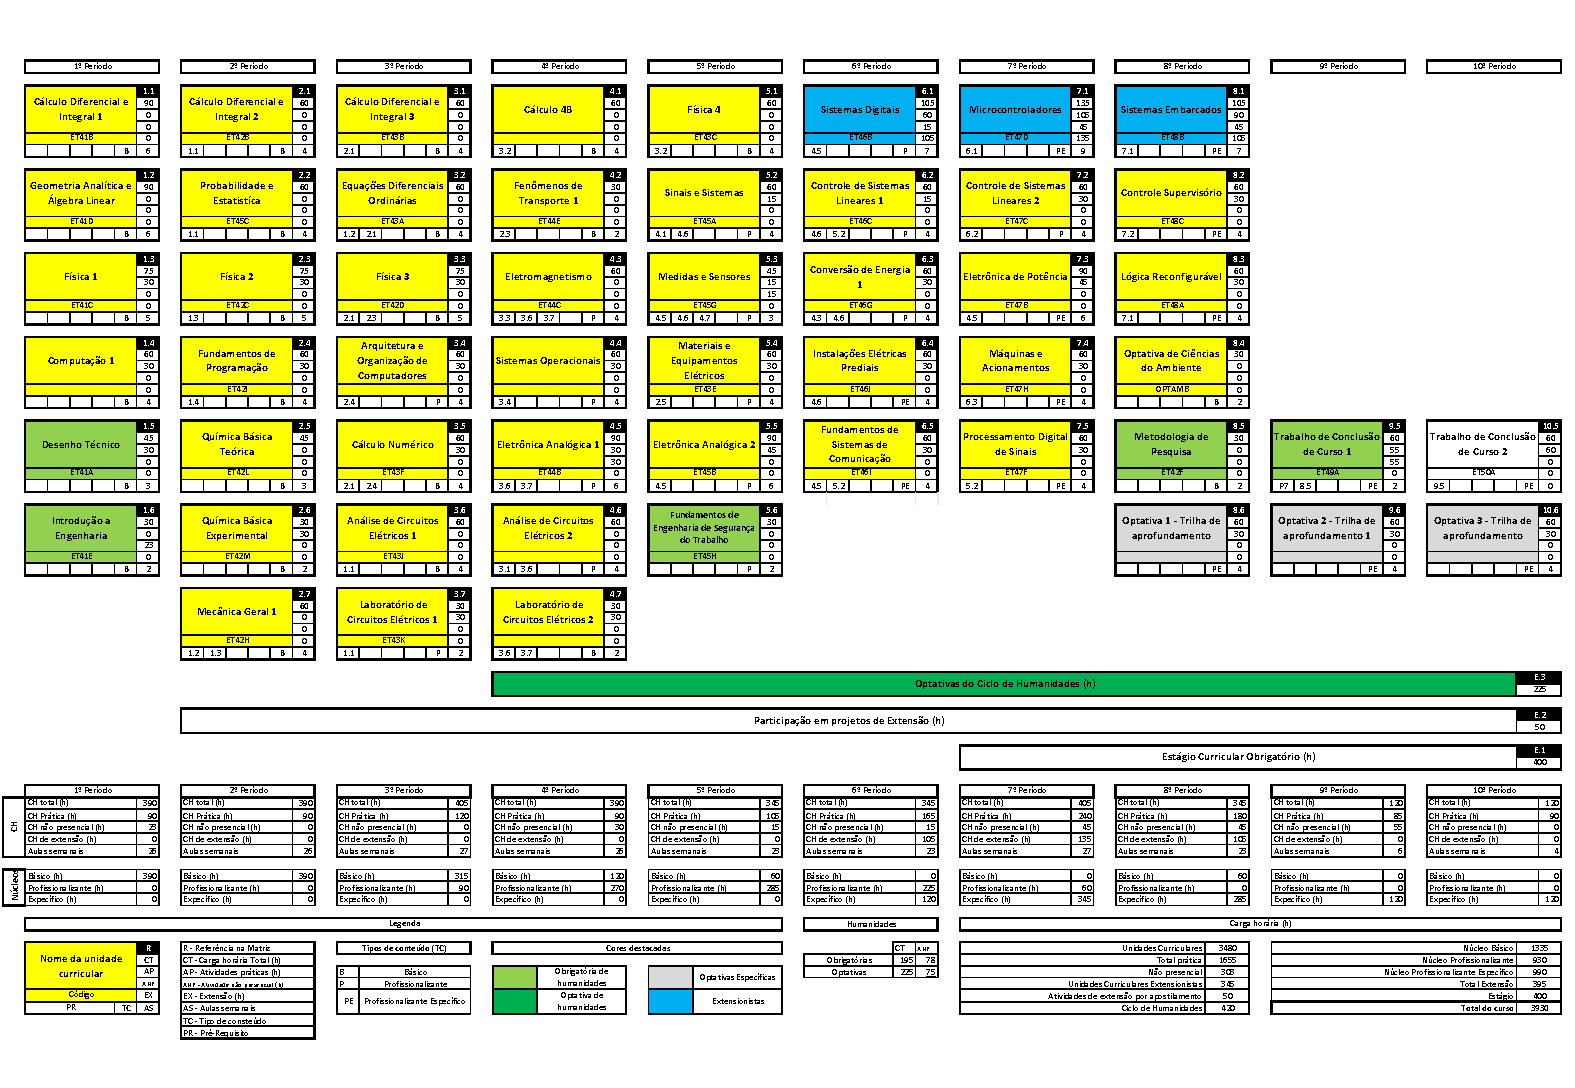
\includegraphics[width=1.3\textwidth]{Caps/Figs/Matriz_final_v2.pdf}
		\fonte{\utf}
		\label{qua:matriz}
	\end{quadro}
\end{landscape}
\restoregeometry



\subsection{Regime Letivo}
\label{sub:reg}

As atividades acadêmicas do curso são de regime semestral, com número mínimo de pré-requisitos, visando melhor consolidação dos conhecimentos nas áreas de atuação do engenheiro eletrônico. A matrícula no curso é realizada por Unidade Curricular. Quanto à matrícula e a periodização serão seguidas as normas institucionais do Regulamento de Organização Didático Pedagógica aplicável ao curso \cite{rodp}.

\subsection{Duração do curso}

O curso de Engenharia Eletrônica possui o período de integralização mínimo em 5 anos (10 períodos, sendo cada período equivalente a um semestre letivo) e máxima em 9 anos (18 semestres), de acordo com o Regulamento da Organização Didático Pedagógica dos Cursos de Graduação da UTFPR \cite{rodp}. A carga horária total é de \the\value{horasT} h. 

Destaca-se que, conforme a Instrução Normativa 02/10 da Instituição \cite{in2:2010:prograd}, uma aula na UTFPR possui 50 minutos. Assim sendo, cada hora das unidade curriculares correspondem a 1,2 aulas. Dessa forma, a cada 15 horas são realizadas 18 aulas.

\subsection{Carga horária de atividades teóricas e práticas}

As atividades teóricas (AT) do curso compreendem \the\value{horasAT} h, correspondendo a \percentagem{\the\value{horasAT}}{\the\value{horasT}} da carga horária total (\the\value{horasT} h). Conforme explicitado na \autoref{sec:matriz}, as ATs correspondem às atividades, de caráter presencial ou não, utilizadas para o desenvolvimento e compreensão de conceitos e de teorias.

\nomenclature[A]{PROGRAD}{Pró-reitoria de Graduação} 

As atividades práticas (AP) do curso compreendem \the\value{horasAP} h, correspondendo a \percentagem{\the\value{horasAP}}{\the\value{horasT}} da carga horária total (\the\value{horasT} h). São atividades de caráter presencial ou não, utilizadas para o desenvolvimento prático de conteúdos, tais como: atividades de laboratório, desenvolvimento de projetos, estudos de caso, visitas técnicas, levantamentos em campo, produção de textos, estágio, trabalho de conclusão de curso, atividades práticas de extensão, dentre outras. Além disso, todo ano é promovida a semana acadêmica com enfoque em atividades científicas, minicursos, atividades de extensão, palestras e seminários com profissionais que atuam em áreas pertinentes à formação do discente e outros. Também são promovidas, de acordo com a disponibilidade, visitas técnicas durante o curso.

\subsection{Carga horária de atividades não presenciais}

As atividades não presenciais (ANP) do curso compreendem \the\value{horasANP} h, correspondendo a \percentagem{\the\value{horasANP}}{\the\value{horasT}} da carga horária total (\the\value{horasT} h). As ANPs são distribuídas em diversas disciplinas estratégicas visando fomentar a cultura de ensino à distância no corpo discente e docente, gerando assim maturidade para esse processo de ensino-aprendizagem. Essa carga horária deve ser planejada pelos docentes, observando, necessariamente, a mediação por Tecnologias da Informação e Comunicação (TICS), assim como atender a regulamentação definida na Resolução nº 39/2019 – COGEP \cite{cogep39}. 

Segundo portaria de MEC N\textordmasculine{} 2.117, de 6 de dezembro de 2019 \cite{portaria2117mec}, as instituições de ensino poderão ofertar disciplinas em no máximo 40\% de sua carga horária total do curso. A principal ferramenta de Tecnologia de informação e comunicação (TIC) para a oferta desta modalidade é o sistema MOODLE. Para que uma disciplina ocorra desta maneira deve estar previsto em plano de ensino e ser aprovado por colegiado competente. Entretanto, em caso de ausência do docente por motivo previsto ou não previsto (como acidentes, doenças, falecimentos, dentre outros) a aula pode ser antecipada ou reposta por meio de uma atividade não presencial a distância desde que seja aprovada pelo coordenador do curso conforme Resolução n\textordmasculine 084/17 do COGEP \cite{cogep84}.

\nomenclature[A]{AD}{Aulas à distência}
\nomenclature[A]{ANPD}{Atividades não presenciais}

\subsection{Carga horária do Estágio Curricular Obrigatório}

Segundo as Diretrizes Curriculares Nacionais dos Cursos de Graduação em Engenharia \cite{dcneng}, em seu artigo 11, ``a formação  do  engenheiro  inclui,  como  etapa  integrante da  graduação, as práticas reais, entre as quais o estágio curricular obrigatório sob supervisão direta do curso''. Aliado a essa diretriz, a UTFPR estabelece, na Resolução COGEP-UTFPR N\textordmasculine{} 142/2022, de 25 de fevereiro de 2022 \cite{cogep142}, que a carga horária mínima de estágio obrigatório para os cursos da UTFPR deve ser de no mínimo \the\value{horasEST}, sendo esse o mesmo valor adotado pelo curso de Engenharia Eletrônica.

\nomenclature[A]{COEMP}{Conselho de Ralações Empresariais e comunitárias}

%\subsection{Carga horária do TCC}

%O TCC tem uma carga total de 144 horas-aula, a carga horária é dividida igualmente nas disciplinas de TCC 1 e TCC 2.

%\subsection{Carga horária de Atividade complementares}

%\pdfmarkupcomment{Verificar se as Atividade complementares continuarão.}{segundo as DCNs, deve-se manter}

\subsection{Carga horária das Atividades de Extensão}
\label{sub:extch}

A curricularização da Extensão no curso, é desenvolvida como uma possibilidade de aplicação de um conjunto de conhecimentos desenvolvidos durante as atividades de ensino e pesquisa e ofertada para a comunidade universitária da UTFPR, à comunidade no entorno direto da Universidade e às regiões circunvizinhas.

As atividades de Extensão enfocam a observação da realidade, tratada com o objetivo de produzir impacto junto à comunidade visando o desenvolvimento regional sustentável. Estarão organizadas em torno de programas ou projetos, sendo incluídas no projeto individual de algumas disciplinas, totalizando \the\value{horasEXT} h, representando \percentagem{\the\value{horasEXT}}{\the\value{horasT}} da carga horária total do curso.

\subsection{Carga horária dos Núcleos de Conteúdos}

Conforme estabelece as Diretrizes Curriculares Nacionais para os cursos Engenharia, existem três núcleos de conteúdo: (i) Básicos; (ii) Profissionalizantes e (iii) Profissionalizantes Específicos. A carga horária desses núcleos no âmbito do curso de Engenharia Eletrônica é mostrada no \autoref{tab:nucleos}.

\begin{table}
	\centering
	\caption[Carga horária dos núcleos de conteúdo]{Carga horária dos núcleos de conteúdo}        
    \label{tab:nucleos}
	\begin{tabularx}{0.7\textwidth}{>{\centering\arraybackslash}X >{\centering\arraybackslash}X >{\centering\arraybackslash}X }\toprule
	\textbf{Núcleo}					& \textbf{Carga horária (h)}	& \textbf{\% da carga horária total}	\\ \midrule 
	Básico							& \the\value{horasB}			& \percentagem{\the\value{horasB}}{\the\value{horasT}}	\\ \rowcolor{gray!10}
	Profissionalizante				& \the\value{horasPR}			& \percentagem{\the\value{horasPR}}{\the\value{horasT}}	\\ 
	Profissionalizante Específico	& \the\value{horasPE}			& \percentagem{\the\value{horasPE}}{\the\value{horasT}}	\\ \bottomrule
	\end{tabularx}
\end{table}

\subsection{Carga horária do ciclo de humanidades}

A fim de contribuir para uma formação mais humanística de seus egressos, os Projetos Pedagógicos dos Cursos de graduação da UTFPR devem estabelecer em sua estrutura curricular um ciclo de humanidades \cite{cogep142}, compreendendo um mínimo de 10$\%$ da carga horária total de unidades curriculares. 

No curso de Engenharia Eletrônica o ciclo de humanidades é estabelecido em \the\value{horasH} h, correspondendo a \percentagem{\the\value{horasH}}{\the\value{horasT}} da carga horária total do curso, ou \percentagem{\the\value{horasH}}{\the\value{horasUC}} da carga horária de unidades curriculares. A estruturação do ciclo de humanidades é demonstrada nas seções \ref{subsec:humanidades} e \ref{subsec:opthumanidades}.

\section{CONTEÚDOS CURRICULARES}

Esta seção descreve os componentes curriculares por período, as unidades curriculares obrigatórias, optativas e eletivas, demonstrando a totalização das cargas horárias.  A composição da distribuição gradual dos períodos e áreas de conhecimento é apresentado em uma sequência didática lógica demonstrando a integração entre os componentes curriculares. Também é descrito como está estruturado o ciclo de humanidades (grupo de unidades curriculares da área de humanidades exigido pela Resolução N\textordmasculine{} 142 COGEP \cite{cogep142}).

\subsection{Unidades Curriculares do Primeiro Período}

Este período do curso, historicamente, apresenta-se como um dos semestres mais difíceis e desafiadores para o corpo discente. Isto pode estar relacionado ao próprio momento em que o discente se encontra, buscando se adaptar a uma nova realidade, muitas das vezes experimentando o conflito entre a gestão da liberdade pessoal e a necessidade de se disciplinar frente às atividades acadêmicas. Em outra perspectiva, a turma do Primeiro Período geralmente apresenta grande diversidade de cultura e formação básica, o que torna importante a implementação de momentos de nivelamento e ambientação que propiciem um melhor fluxo de desenvolvimento das disciplinas e, consequentemente, seu melhor aproveitamento.

Desta forma, o Primeiro Período possui disciplinas que buscam e ambientar o discente ao curso, tais como ``Introdução à Engenharia'' e ``Computação 1''.

Adicionalmente, este período é o início do alicerce para as fundamentações matemáticas necessárias para o bom engenheiro eletrônico. Essa fundamentação se estende até o quarto período onde, a partir de então, as unidades curriculares específicas e profissionalizantes se iniciam.

%As unidades curriculares do Primeiro Período são \listaUC{1}{Dados/unidadesCurriculares.csv}, totalizando \the\value{horasP1} h. A \autoref{tab:per1} representa a distribuição das unidades curriculares do primeiro período do curso de Engenharia Eletrônica. Dessa forma,\listaUC{1}{Dados/unidadesCurriculares.csv}, totalizam \the\value{horasP1} h.

Os conteúdos curriculares do primeiro período estão listados na \autoref{tab:per1}. Adicionalmente, a estrutura de cada unidade curricular é apresentada em quadros: \listaUC{1}{Dados/unidadesCurriculares.csv}.

% tabela de unidades curriculares do primeiro período
\begin{table}[!htb]
	\centering\footnotesize
	\caption{Conteúdos curriculares do Primeiro Período}
	\label{tab:per1}
	\tabelaPeriodo{1}{Dados/unidadesCurriculares.csv}
	\fonte{Autoria própria}
\end{table}

\imprimeEmentas{1}{Dados/unidadesCurriculares.csv}\clearpage



\subsection{Unidades Curriculares do Segundo Período}

Os conteúdos curriculares do segundo período estão listados na \autoref{tab:per2}. Adicionalmente, a estrutura de cada unidade curricular é apresentada em quadros: \listaUC{2}{Dados/unidadesCurriculares.csv}.

% tabela de unidades curriculares do segundo período
\begin{table}[!htb]
	\centering\footnotesize
	\caption{Conteúdos curriculares do Segundo Período}
	\label{tab:per2}
	\tabelaPeriodo{2}{Dados/unidadesCurriculares.csv}
	\fonte{Autoria própria}
\end{table}

\imprimeEmentas{2}{Dados/unidadesCurriculares.csv}\clearpage

\subsection{Unidades Curriculares do Terceiro Período}

Os conteúdos curriculares do terceiro período estão listados na \autoref{tab:per3}. Adicionalmente, a estrutura de cada unidade curricular é apresentada em quadros: \listaUC{3}{Dados/unidadesCurriculares.csv}.

% tabela de unidades curriculares do terceiro período
\begin{table}[!htb]
	\centering\footnotesize
	\caption{Conteúdos curriculares do Terceiro Período}
	\label{tab:per3}
	\tabelaPeriodo{3}{Dados/unidadesCurriculares.csv}
	\fonte{Autoria própria}
\end{table}

\imprimeEmentas{3}{Dados/unidadesCurriculares.csv}\clearpage

\subsection{Unidades Curriculares do Quarto Período}

Os conteúdos curriculares do quarto período estão listados na \autoref{tab:per4}. Adicionalmente, a estrutura de cada unidade curricular é apresentada em quadros: \listaUC{4}{Dados/unidadesCurriculares.csv}.

% tabela de unidades curriculares do quarto período
\begin{table}[!htb]
	\centering\footnotesize
	\caption{Conteúdos curriculares do Quarto Período}
	\label{tab:per4}
	\tabelaPeriodo{4}{Dados/unidadesCurriculares.csv}
	\fonte{Autoria própria}
\end{table}

\imprimeEmentas{4}{Dados/unidadesCurriculares.csv}\clearpage

\subsection{Unidades Curriculares do Quinto Período}

Os conteúdos curriculares do quinto período estão listados na \autoref{tab:per5}. Adicionalmente, a estrutura de cada unidade curricular é apresentada em quadros: \listaUC{5}{Dados/unidadesCurriculares.csv}.

% tabela de unidades curriculares do quinto período
\begin{table}[!htb]
	\centering\footnotesize
	\caption{Conteúdos curriculares do Quinto Período}
	\label{tab:per5}
	\tabelaPeriodo{5}{Dados/unidadesCurriculares.csv}
	\fonte{Autoria própria}
\end{table}

\imprimeEmentas{5}{Dados/unidadesCurriculares.csv}\clearpage

\subsection{Unidades Curriculares do Sexto Período}

Os conteúdos curriculares do sexto período estão listados na \autoref{tab:per6}. Adicionalmente, a estrutura de cada unidade curricular é apresentada em quadros: \listaUC{6}{Dados/unidadesCurriculares.csv}.

% tabela de unidades curriculares do sexto período
\begin{table}[!htb]
	\centering\footnotesize
	\caption{Conteúdos curriculares do Sexto Período}
	\label{tab:per6}
	\tabelaPeriodo{6}{Dados/unidadesCurriculares.csv}
	\fonte{Autoria própria}
\end{table}

\imprimeEmentas{6}{Dados/unidadesCurriculares.csv}\clearpage

\subsection{Unidades Curriculares do Sétimo Período}

Os conteúdos curriculares do sétimo período estão listados na \autoref{tab:per7}. Adicionalmente, a estrutura de cada unidade curricular é apresentada em quadros: \listaUC{7}{Dados/unidadesCurriculares.csv}.

% tabela de unidades curriculares do sétimo período
\begin{table}[!htb]
	\centering\footnotesize
	\caption{Conteúdos curriculares do Sétimo Período}
	\label{tab:per7}
	\tabelaPeriodo{7}{Dados/unidadesCurriculares.csv}
	\fonte{Autoria própria}
\end{table}

\imprimeEmentas{7}{Dados/unidadesCurriculares.csv}\clearpage

\subsection{Unidades Curriculares do Oitavo Período}

Os conteúdos curriculares do oitavo período estão listados na \autoref{tab:per8}. Adicionalmente, a estrutura de cada unidade curricular é apresentada em quadros: \listaUC{8}{Dados/unidadesCurriculares.csv}.

% tabela de unidades curriculares do oitavo período
\begin{table}[!htb]
	\centering\footnotesize
	\caption{Conteúdos curriculares do Oitavo Período}
	\label{tab:per8}
	\tabelaPeriodo{8}{Dados/unidadesCurriculares.csv}
	\fonte{Autoria própria}
\end{table}

\imprimeEmentas{8}{Dados/unidadesCurriculares.csv}\clearpage

\subsection{Unidades Curriculares do Nono Período}

Os conteúdos curriculares do nono período estão listados na \autoref{tab:per9}. Adicionalmente, a estrutura de cada unidade curricular é apresentada em quadros: \listaUC{9}{Dados/unidadesCurriculares.csv}.

% tabela de unidades curriculares do nono período
\begin{table}[!htb]
	\centering\footnotesize
	\caption{Conteúdos curriculares do Nono Período}
	\label{tab:per9}
	\tabelaPeriodo{9}{Dados/unidadesCurriculares.csv}
	\fonte{Autoria própria}
\end{table}

\imprimeEmentas{9}{Dados/unidadesCurriculares.csv}\clearpage

\subsection{Unidades Curriculares do Décimo Período}

Os conteúdos curriculares do décimo período estão listados na \autoref{tab:per10}. Adicionalmente, a estrutura de cada unidade curricular é apresentada em quadros: \listaUC{10}{Dados/unidadesCurriculares.csv}.

% tabela de unidades curriculares do décimo período
\begin{table}[!htb]
	\centering\footnotesize
	\caption{Conteúdos curriculares do Décimo Período}
	\label{tab:per10}
	\tabelaPeriodo{10}{Dados/unidadesCurriculares.csv}
	\fonte{Autoria própria}
\end{table}

\imprimeEmentas{10}{Dados/unidadesCurriculares.csv}\clearpage

O Décimo período, assim como o nono, foram concebidos com poucas unidades curriculares (semipresenciais da trilha de aprofundamento), para que o discente possa finalizar o TCC, realizar o Estágio Curricular Obrigatório e integralizar as atividades de extensão.

O curso apresenta um máximo de \the\value{horasANP} horas em carga horária não presencial, distribuídas em diversas disciplinas. Essa carga horária deve ser planejada pelos docentes, observando, necessariamente, a mediação por Tecnologias da Informação e Comunicação (TICS), assim como atender a regulamentação definida na Resolução n\textordmasculine{} 39/2019 – COGEP \cite{cogep39}. A estratégia adotada contempla a combinação de ambientes físicos com ambientes digitais de aprendizagem, focados no desenvolvimento de projetos ou trabalhos práticos.

\subsection{Unidades Curriculares Optativas - Ciências do Ambiente}

O discente matriculado no curso de Engenharia Eletrônica deve cursar no mínimo 30 h de unidades curriculares de Ciências Ambientais. As unidades curriculares optativas de Ciências Ambientais estão listadas na \autoref{tab:per41}. Adicionalmente, a estrutura de cada unidade curricular é apresentada em quadros: \listaUC{41}{Dados/unidadesCurriculares.csv}. %Os dados estruturais das unidades curriculares estão nos quandros \ref{qua:ucCA78A}, \ref{qua:ucCA78B} e \ref{qua:ucCA78C}.

\begin{table}[!htb]
	\centering\footnotesize
	\caption{Conteúdos curriculares de Ciências Ambientais}
	\label{tab:per41}
	\tabelaTrilha{41}{Dados/unidadesCurriculares.csv}
	\fonte{Autoria própria}
\end{table}

\imprimeEmentasOpt{41}{Dados/unidadesCurriculares.csv}\clearpage



\subsection{Unidades Curriculares Optativas - Trilhas}
\label{subsec:trilhas}

As Trilhas de Aprofundamento foram concebidas como fator para flexibilização da matriz curricular, facilitador da mobilidade acadêmica e internacionalização e desenvolvimento de áreas de aprofundamento estratégicas para o curso, que foram escolhidas para atender o arranjo produtivo regional, bem como sintonizar a formação com o contexto tecnológico contemporâneo.

% Trilha de Controle e Automação
\subsubsection{Trilha de Controle e Automação}

Os conteúdos curriculares da Trilha de Controle e Automação estão listados na \autoref{tab:per21}. Adicionalmente, a estrutura de cada unidade curricular é apresentada em quadros: \listaUC{21}{Dados/unidadesCurriculares.csv}.

% tabela de unidades curriculares da Trilha de Controle e Automação
\begin{table}[!htb]
	\centering\footnotesize
	\caption{Conteúdos curriculares da trilha de Controle e Automação}
	\label{tab:per21}
	\tabelaTrilha{21}{Dados/unidadesCurriculares.csv}
	\fonte{Autoria própria}
\end{table}

\imprimeEmentasOpt{21}{Dados/unidadesCurriculares.csv}\clearpage

% Trilha de Computação
\subsubsection{Trilha de Computação}

Os conteúdos curriculares da Trilha de Computação estão listados na \autoref{tab:per22}. Adicionalmente, a estrutura de cada unidade curricular é apresentada em quadros: \listaUC{22}{Dados/unidadesCurriculares.csv}.

% tabela de unidades curriculares da Trilha de Computação
\begin{table}[!htb]
	\centering\footnotesize
	\caption{Conteúdos curriculares da trilha de Computação}
	\label{tab:per22}
	\tabelaTrilha{22}{Dados/unidadesCurriculares.csv}
	\fonte{Autoria própria}
\end{table}

\imprimeEmentasOpt{22}{Dados/unidadesCurriculares.csv}\clearpage

% Trilha de Eletrônica
\subsubsection{Trilha de Eletrônica}

Os conteúdos curriculares da Trilha de Eletrônica estão listados na \autoref{tab:per23}. Adicionalmente, a estrutura de cada unidade curricular é apresentada em quadros: \listaUC{23}{Dados/unidadesCurriculares.csv}.

% tabela de unidades curriculares da Trilha de Eletrônica
\begin{table}[!htb]
	\centering\footnotesize
	\caption{Conteúdos curriculares da trilha de Eletrônica}
	\label{tab:per23}
	\tabelaTrilha{23}{Dados/unidadesCurriculares.csv}
	\fonte{Autoria própria}
\end{table}

\imprimeEmentasOpt{23}{Dados/unidadesCurriculares.csv}\clearpage

% Trilha de Eletrotécnica
\subsubsection{Trilha de Eletrotécnica}

Os conteúdos curriculares da Trilha de Eletrotécnica estão listados na \autoref{tab:per24}. Adicionalmente, a estrutura de cada unidade curricular é apresentada em quadros: \listaUC{24}{Dados/unidadesCurriculares.csv}.

% tabela de unidades curriculares da Trilha de Eletrotécnica
\begin{table}[!htb]
	\centering\footnotesize
	\caption{Conteúdos curriculares da trilha de Eletrotécnica}
	\label{tab:per24}
	\tabelaTrilha{24}{Dados/unidadesCurriculares.csv}
	\fonte{Autoria própria}
\end{table}

\imprimeEmentasOpt{24}{Dados/unidadesCurriculares.csv}\clearpage

\subsection{O ciclo de Humanidades}
\label{subsec:humanidades}

De acordo com a Resolução COGEP/UTFPR N\textordmasculine{} 142, de 25 de fevereiro de 2022 \cite{cogep142}:

\begin{citacao}
	``os PPCs de graduação da UTFPR devem estabelecer em sua estrutura curricular, a partir do disposto nas DCNs, um ciclo de humanidades, representando uma carga horária igual ou superior a 10$\%$ (dez por cento) da carga horária total destinada às unidades curriculares do curso.''

\end{citacao}

Ainda segundo a referida Resolução: 

\begin{citacao}
	``o ciclo de humanidades será composto pelas áreas de ciências humanas, pela área de ciências sociais aplicadas e pela área de linguística, letras e artes, podendo incluir também, unidades/componentes curriculares na área de atividade física, saúde e qualidade de vida.''
\end{citacao}

Para a composição do ciclo de humanidades, a Resolução COGEP/UTFPR N\textordmasculine{} 142 estabelece os seguintes componentes:

\begin{enumerate}
	\item componentes da área de ciências humanas: antropologia, arqueologia, educação, filosofia, geografia, história, psicologia, sociologia, ciência política, relações internacionais e teologia, incluindo suas subáreas;
	\item componentes da área de ciências sociais aplicadas: administração, arquitetura e urbanismo, ciência da informação, direito, economia, planejamento urbano e regional, demografia, serviço social, turismo, desenho industrial, museologia e comunicação, incluindo suas subáreas;
	\item componentes da área de linguística, letras e artes: linguística, letras e artes, incluindo suas subáreas; e
	\item IV - atividade física, saúde e qualidade de vida.
\end{enumerate}

Dessa forma, o curso de Engenharia Eletrônica contempla em sua matriz um ciclo de humanidades composto por unidades curriculares obrigatórias e optativas, que representam \percentagem{\the\value{horasH}}{\the\value{horasUC}} da carga horária de unidades curriculares do curso. 


\subsection{Unidades Curriculares do Ciclo de Humanidades}
\label{subsec:obghumanidades}

A \autoref{tab:obghum}, mostra a relação das unidades curriculares obrigatórias do ciclo de humanidades junto com as respectivas áreas estabelecidas na Resolução COGEP/UTFPR N\textordmasculine{} 142 \cite{cogep142}. Também mostra, o quantitativo de carga horária de unidades curriculares optativas.

% tabela de unidades curriculares optativas de humanidades
\begin{table}[!htb]
	\centering\footnotesize
	\caption{Unidades curriculares de humanidades}
	\label{tab:obghum}
	\tabelaHum{Dados/unidadesCurriculares.csv}
	\fonte{Autoria própria}
\end{table}

\subsection{Unidades Curriculares Optativas do Ciclo de Humanidades}
\label{subsec:opthumanidades}

Os conteúdos curriculares optativos de Humanidades estão listados na \autoref{qua:ucHUM}, juntamente com as respectivas áreas estabelecidas na Resolução COGEP/UTFPR N\textordmasculine{} 142 \cite{cogep142}. Adicionalmente, a estrutura de cada unidade curricular é apresentada em quadros: \listaUC{31}{Dados/unidadesCurriculares.csv}.

% tabela de unidades curriculares optativas de humanidades
\begin{table}[!htb]
	\centering\footnotesize
	\caption{Conteúdos curriculares optativos de humanidades}
	\label{qua:ucHUM} % Não alterar
	\tabelaOptHum{31}{Dados/unidadesCurriculares.csv}
	\fonte{Autoria própria}
\end{table}

Para integralizar o ciclo de humanidades, o discente matriculado no curso de Engenharia Eletrônica deve cursar no mínimo 90 h da área de linguística e letras e 135 h nas demais áreas.

\imprimeEmentasHum{31}{Dados/unidadesCurriculares.csv}\clearpage


\section{O Estágio Curricular Obrigatório}

O Estágio Curricular Supervisionado deve oferecer condições suficientes para que o aluno possa, de acordo com o PDI \cite{pdiutfpr}, inserir-se com maior facilidade no mercado de trabalho. O PDI destaca:

\begin{citacao}
	``o estágio curricular é obrigatório para todos os cursos de nível técnico e de graduação, visa à complementação do processo ensino-aprendizagem e tem como objetivos: (i) facilitar a futura inserção do estudante no mundo de trabalho; (ii) servir como mecanismo de relacionamento entre a UTFPR e as entidades concedentes de estágio; e (iii) propiciar a adaptação social e psicológica do estudante à futura atividade profissional''.
\end{citacao}

%\dadoCHT{E.1}

O estágio como previsto na Lei nº 11.788, de 25 de setembro de 2008 \cite{Lei:11788:2008} é o ato educativo escolar supervisionado, desenvolvido no ambiente de trabalho, no qual visa a preparação do estudante para o ingresso no mercado de trabalho, facilitando a adaptação social e psicológica à futura atividade profissional do estudante. Além disso, busca-se o aprendizado de competências próprias da atividade profissional e a contextualização curricular, objetivando o desenvolvimento do educando para a vida cidadã e para o trabalho.

O estágio poderá ser realizado em organizações públicas, privadas ou do terceiro setor, que apresentem condições de proporcionar experiência prática na área de formação do estudante, podendo, também, proporcionar o desenvolvimento sócio cultural ou científico, pela participação em situações de vida e de trabalho no seu meio. O estágio pode ser realizado de duas formas:

\begin{itemize}
	\item Estágio Curricular Obrigatório: é aquele definido como tal no PPC, cuja carga horária é requisito para aprovação e obtenção de diploma;
	\item Estágio Não Obrigatório: é aquele desenvolvido como atividade opcional, acrescida à carga horária regular e obrigatória.
\end{itemize}

O Estágio Curricular Obrigatório é considerado disciplina/unidade curricular obrigatória dos cursos regulares do Ensino Superior da UTFPR. O Estágio Curricular Obrigatório deve ser planejado, executado, acompanhado e avaliado em conformidade com os currículos, programas e calendários acadêmicos. Poderá ser matriculado na disciplina/unidade curricular de Estágio Curricular Obrigatório o estudante que estiver regularmente matriculado na UTFPR a partir do 7\textordmasculine{} (sétimo) período do curso.

O Estágio Curricular Obrigatório tem duração mínima de \dadoCHT{E.1} h, podendo ser desenvolvido em mais de uma Unidade Concedente de Estágio (UCE), sendo que a atuação do estudante em cada uma delas não deverá ser inferior a 100 h. A jornada diária do estágio será compatível com o horário escolar do estudante, devendo constar no termo de compromisso e não ultrapassar 6 h diárias e 30 h semanais. Adicionalmente, nos períodos em que não estão programadas aulas presenciais os alunos poderão realizar estágio com carga horária de até 8 h diárias e 40 h semanais. O acompanhamento das atividades do estagiário deve ser feito pela UCE por meio da indicação de um funcionário supervisor, com formação ou experiência na área; pelo professor responsável pela atividade de estágio (PRAE) e pelo professor orientador.

O estudante que exercer atividade profissional correlata ao seu curso na condição de empregado devidamente registrado, autônomo ou empresário, ou ainda atuando oficialmente em programas de incentivo à pesquisa científica, ao desenvolvimento tecnológico, poderá valer-se de tais atividades para efeitos de realização do seu Estágio Curricular Obrigatório, desde que atendam ao PPC.

As atividades de Estágio Não Obrigatório podem ser iniciadas a partir do segundo semestre e durante todo o curso, com exceção do período de realização do Estágio Curricular Obrigatório, através de convênios ou projetos firmados entre a Universidade e UCE. O Estágio será precedido da celebração do instrumento jurídico entre o estudante e a UCE, com interveniência da UTFPR, por meio da Diretoria de Relações Empresariais e Comunitárias (DIREC).

Os procedimentos para a realização e acompanhamento de estágios nos Cursos de Educação Profissional Técnica de Nível Médio e no Ensino Superior da UTFPR são estabelecidos pela Resolução Conjunta N\textordmasculine{} 01/2020, de 02 de junho de 2020 \cite{cogepcoemp1:2020}.

% Colocar a norma do curso assim que for publicada

\section{Trabalho de conclusão de curso}

O Trabalho de Conclusão de Curso (TCC) é um componente curricular obrigatório para os cursos de graduação \cite{dcneng}. No ambito da UTFPR, o TCC deve atender à resolução n\textordmasculine 18/2018 – COGEP, Regulamento do Trabalho de Conclusão de Curso (TCC) para os Cursos de Graduação da UTFPR \cite{cogep18}. Os objetivos do TCC são:

\begin{enumerate}
	\item Desenvolver a capacidade de aplicação dos conceitos e teorias adquiridas durante o curso de forma integrada;
	\item Desenvolver a capacidade de planejamento e disciplina para resolver problemas dentro das diversas áreas de formação;
	\item Despertar o interesse pela aplicação do conhecimento como meio para a resolução de problemas;
	\item Estimular o espírito empreendedor, por meio de desenvolvimento de projetos;
	\item Intensificar a extensão universitária, por intermédio da resolução de problemas e identificação de oportunidades existentes nos diversos setores da sociedade;
	\item Desenvolver a capacidade de análise e de busca de soluções para problemas sociais, políticos, tecnológicos, ambientais, éticos e metodológicos;
	\item Estimular a construção do conhecimento coletivo; 
	\item Estimular a inter, multi e transdisciplinaridade;
	\item Estimular a inovação tecnológica, através da transferência de tecnologia, desenvolvimento de patentes e/ou comercialização dos resultados;
	\item Estimular a articulação entre ensino e pesquisa.  
		
\end{enumerate}

O TCC está dividido em duas etapas: TCC 1 e TCC 2, onde cada etapa contempla 60 h. O objetivo final no TCC 1 é a elaboração de um projeto de pesquisa e defendê-lo frente a uma banca avaliadora, incluindo o professor orientador. O TCC 2 tem como objetivo a execução desse projeto de pesquisa e sua defesa pública, conforme regulamento acima citado e normas complementares de TCC do curso de Engenharia Eletrônica campus Toledo, aprovadas em colegiado.

As atividades de TCC do curso são coordenadas por um Professor Responsável pela atividade de TCC (PRATCC) indicado pelo coordenador do curso. Cabe a esse professor constituir as bancas de avaliação e apoiar as diversas atividades relativas a TCC. O acompanhamento dos alunos no TCC é efetuado por um Professor Orientador, indicado pelo Professor Responsável pelo TCC. O detalhamento das atividades de TCC, bem como das responsabilidades dos envolvidos, podem ser obtidas na norma geral de TCC da UTFPR \cite{cogep18}.

\section{Síntese de distribuição de carga horária}

A \autoref{tab:ch} sumariza as cargas horárias do curso, indicando os totais para o Ciclo de Humanidades, atividades de extensão, TCC e para as atividades não presenciais. Os percentuais de cada total é calculado em relação a carga horária total do curso (\the\value{horasT} h).

É possível notar, através da referida tabela, que o curso atende à Resolução CNE/CES N\textordmasculine{} 7, de 18 de dezembro de 2018, que determina um mínimo de 10$\%$ da carga horária do curso, voltada para atividades extensionistas.

\begin{table}[!htb]
	\rowcolors{3}{white}{tableShade}
	\centering
	\caption{Síntese de distribuição de carga horária do curso de Engenharia Eletrônica}
	\label{tab:ch}
	\begin{tabularx}{\textwidth}{c|>{\centering\arraybackslash}X | >{\centering\arraybackslash}X | c} \toprule%\hiderowcolors
		\bfseries Item		& \bfseries Atividade										& \bfseries Carga Horária (h) 	&	\bfseries Composição$^1$	\\	\midrule \midrule
		a = d + f + i		& Integralização / Carga horária Total						& \the\value{horasT}			&	100$\%$			\\			
		b					& Unidades Curriculares Optativas							& \the\value{horasOPT}			&	\percentagem{\the\value{horasOPT}}{\the\value{horasT}}				\\	
		c					& Unidades Curriculares Obrigatórias						& \the\value{horasOBG}			&	\percentagem{\the\value{horasOBG}}{\the\value{horasT}}				\\	
		d = c + d			& Unidades Curriculares										& \the\value{horasUC}			&	\percentagem{\the\value{horasUC}}{\the\value{horasT}}				\\	
		e					& Unidades Curriculares extensionistas						& \the\value{horasUCEXT}		&	\percentagem{\the\value{horasUCEXT}}{\the\value{horasT}}			\\	
		f					& Atividades extensionistas complementares / Apostilamento	& \the\value{horasCEXT}			&	\percentagem{\the\value{horasCEXT}}{\the\value{horasT}}				\\	
		g = e + f			& Atividades extensionistas 								& \the\value{horasEXT}			&	\percentagem{\the\value{horasEXT}}{\the\value{horasT}}				\\	
		h					& Ciclo de Humanidades 										& \the\value{horasH}			&	\percentagem{\the\value{horasH}}{\the\value{horasT}}$^2$				\\	
		i					& Estágio 													& \the\value{horasEST}			&	\percentagem{\the\value{horasEST}}{\the\value{horasT}}				\\	
		j					& Não presencial 											& \the\value{horasANP}			&	\percentagem{\the\value{horasANP}}{\the\value{horasT}}				\\	
		l					& Trabalho de Conclusão de Curso							& 120							&	\percentagem{120}{\the\value{horasT}}				\\	\bottomrule
		
	\end{tabularx}
	\begin{tabularx}{\textwidth}{l}
		\hiderowcolors
		\tiny $^1$ - Porcentagem em relação à carga horária Total\\
		\tiny $^2$ - Representa \percentagem{\the\value{horasH}}{\the\value{horasUC}} da carga horária das unidades curriculares.
	\end{tabularx}
\end{table}

Ademais, as diretrizes curriculares dos cursos de graduação regulares da UTFPR \cite{cogep142} determinam que os PPCs de cursos de graduação da UTFPR devem estabelecer em sua estrutura curricular, a partir do disposto nas DCNs \cite{dcneng}, o ciclo de humanidades, representando uma carga horária igual ou superior a 10$\%$ (dez por cento) da carga horária total destinada às unidades curriculares do curso. Dessa forma, o curso de Engenharia Eletrônica, estabelece \the\value{horasH} h de unidades curriculares humanísticas, representando \percentagem{\the\value{horasH}}{\the\value{horasUC}} da carga horária das unidades curriculares.

\section{Processo de ensino e aprendizagem}

O processo de como o docente trata o ensino e a aprendizagem relaciona-se com uma serie de questionamentos sobre a própria definição do que é aprender e ensinar. Dessa forma, é necessário que os educadores sejam capazes de entender as diferenças de cada atividade e procurar escolher a melhor maneira que irá desenvolver um determinado tema. 

\subsection{Metodologias de aprendizagem}

As metodologias de aprendizagem aplicada no curso de Engenharia Eletrônica são formas de organizar o ensino do discente visando obter o melhor desempenho para atingir o perfil do egresso. Trata-se do ``caminho'' a seguir para conseguir entender e internalizar todo o conhecimento passado. Dessa forma, as metodologias aplicadas estão intimamente relacionadas ao desenvolvimento das competências profissionais apresentadas na \autoref{sec:perf}. As competências são desenvolvidas gradativamente em várias unidades curriculares e em momentos distintos no decorrer do curso, assim como é explicado na \autoref{sec:comp}.

Ao docente atuante no curso de Engenharia Eletrônica é dada a liberdade da escolha da metodologia a ser empregada nas ações de ensino. Esse processo é acompanhado pelo NDE e pelo Departamento de Educação (DEPED-TD), sempre visando o melhor aproveitamento do discente. Neste sentido, a UTFPR dispõe de um Programa de Desenvolvimento Profissional Docente da UTFPR, aprovado pela Resolução COGEP N\textordmasculine{} 32/2019 \cite{cogep32}, com finalidade do aperfeiçoamento da prática docente, possibilitando a busca de alternativas às dificuldades que envolvem os processos de ensino e aprendizagem na Instituição.

São exemplos de metodologias que podem ser empregadas:

\begin{itemize}
	\item Metodologias ativas: o aluno é o principal responsável pelo aprendizado do conteúdo através da participação, interagindo e pensando para aumentar a absorção. Pode-se utilizar estudos de caso, projetos práticos e debates entre equipes de discentes. É o contrario da metodologia passiva, onde o discente apenas assiste as aulas expositivas e depois é avaliado através de provas e trabalhos;
	\item Método de aprendizagem interativo: existe iteração entre o aluno e objeto de estudo, prendendo a atenção do estudante e aprimorando o processo de aprendizagem, como é o caso dos jogos, desafios, animações e atividades práticas de laboratório;
	\item Método de autoaprendizagem: o discente tem liberdade nos estudos, sendo o responsável por gerir o tempo de dedicação na objeto estudado. A dependência de outros profissionais é minimizada, podendo existir a sugestão ou seleção de um bom material de ensino. Esse método é bastante comum nas práticas onde existe um docente orientador de projetos práticos, como é o caso de TCC, IC, IT e trabalhos extraclasse de disciplina.
\end{itemize}



\subsection{Tecnologias de Informação e Comunicação (TICs)}

A instituição disponibiliza alguns ambientes e artefatos de comunicação para mediarem atividades didáticas nas modalidades presencial e não presencial:

\begin{itemize}
    \item Página pessoal docente;
    \item Moodle institucional;
    \item Plataforma GSuite for Education;
    \item Serviço Mconf em parceria com a Rede Nacional de Ensino e Pesquisa (RNP);
    \item Base Digital de dados;
    \item Repositórios institucionais;
    \item Office 365;
    \item Equipamentos de áudio e vídeo em geral.
\end{itemize}
    
Diante disso, o processo de ensino aprendizagem é intensificado com o uso das TICs e demais artefatos tecnológicos, por meio de atividades de comunicação, colaboração e compartilhamento, propiciando a construção e a produção de conhecimentos e o desenvolvimento de habilidades pessoais e interpessoais do corpo discente, e fomentando novas práticas do docente.

Mais informação sobre a utilização de TICs nos processos de ensino e aprendizagem no ambito do curso de Engenharia Eletrônica podem ser encontrados na \autoref{sec:tic}.

\subsection{Processos de avaliação}

O Curso tem como horizonte formar pessoas com capacidade de se expressarem escrita e oralmente, que desenvolvam trabalhos em equipes multidisciplinares, que compreendam e utilizem novas ideias e tecnologias para a resolução de problemas, e os procedimentos de avaliação do processo de ensino-aprendizagem utilizados no curso partem desse pressuposto. São diversificados, elaborados de acordo com a especificidade de cada disciplina, buscando levar em consideração o profissional que se quer formar.

A avaliação do processo de ensino-aprendizagem parte dos objetivos das disciplinas e não negligencia instrumentos como provas escritas, trabalhos de pesquisa bibliográfica, produção de artigos, etc. Por outro lado, há o interesse que se desenvolva no interior das disciplinas, atividades que articulem diferentes áreas do curso, que busquem desenvolver materiais de trabalho que expressem a reflexão sobre problemáticas da sociedade, entre outras questões importantes para o profissional da área.

Mesmo com a realização das provas individuais busca-se diversificar, com a contribuição das Tecnologias de Informação e Comunicação – TICs. Estas podem ser utilizadas em disciplinas como a Estatística e Desenho Técnico, quando softwares computacionais são empregados para a resolução de questões; e a plataforma MOODLE como veículo para a realização de avaliações. A proposição de trabalhos de pesquisa sobre conteúdo específicos e sua formação em editores de texto é uma prática comum ao longo das disciplinas.

No entanto, o emprego de provas individuais para verificar se os objetivos da disciplina foram atingidos, é apenas um dos instrumentos utilizados para avaliar os discentes ao longo do curso e no interior das unidades curriculares. Há a preocupação em avaliar a capacidade do discente em desenvolver seus trabalhos com criatividade, autonomia, flexibilidade e conhecimento vinculando conteúdos para propiciar uma experiência multidisciplinar. 

Com essas estratégias, todas as unidades curriculares do curso utilizam diferentes instrumentos de avaliação, não se resumindo às provas escritas. Além disso, propicia que o acadêmico seja avaliado em diferentes momentos, ao mesmo tempo em que exige diversificados critérios de avaliação. 

Tentando contribuir para a concretização disso, há um cuidado na aprovação dos planos de ensino das unidades curriculares, para que elas expressem claramente os critérios e os instrumentos de avaliação utilizados. O docente da disciplina tem autonomia para estabelecer os pesos específicos para os diferentes instrumentos utilizados. No entanto, é incentivado pelo grupo a utilizar diferentes instrumentos e critérios de avaliação. 

A avaliação da aprendizagem dos discentes por componente curricular, levando-se em consideração a assiduidade e o aproveitamento nos estudos, é realizada de acordo com as especificações referidas no Regulamento da Organização Didático-Pedagógica dos Cursos de Graduação da UTFPR (Resolução n\textordmasculine{} 81/2019 - COGEP, de 26 de julho de 2019 \cite{rodp}) em seu capítulo VI (Do Ensino, do Rendimento escolar e da Aprovação) que segue as seguintes diretrizes: 

\begin{itemize}
	\item Avaliação: número de avaliações não menor do que 2 (duas), onde suas modalidades e critérios devem ser explicitados no Planejamento de Aulas da unidade curricular. Além disso, o docente deverá possibilitar a reavaliação ao longo e/ou ao final do semestre letivo a todos os estudantes matriculados na unidade curricular, oportunizando ao estudante alcançar nota final para aprovação.
	\item Aprovação: frequência igual ou superior a 75$\%$ (setenta e cinco por cento) das aulas presenciais dadas e Nota Final igual ou superior a 6,0 (seis), ou frequência igual ou superior a 50$\%$ (cinquenta por cento) das aulas presenciais dadas e Nota Final igual ou superior a 8,0 (oito);
	\item Aproveitamento: os alunos serão avaliados através de atividades que resultem na avaliação do conhecimento por atribuição de notas a critério do professor e segundo o plano de ensino da disciplina. A flexibilização do regimento da Instituição permite que o professor possa alterar os critérios propostos conforme a necessidade de cada disciplina;
	\item  Condições especiais: pela Resolução n\textordmasculine{} 110/2021 – COGEP \cite{cogep110}, tem-se também o regulamento que estabelece normas para as atividades de acompanhamento domiciliar, abono de faltas, compensação de faltas, dispensa de frequência e lançamento de faltas para os cursos presenciais de nível médio e superior da UTFPR em que situações diversas são consideradas permitindo uma melhor flexibilização do processo de avaliação discente.
\end{itemize}

\subsection{Avaliação dos discentes com necessidades especiais}

Os discentes com necessidades especiais apresentam características e particularidades que não podem ser tratadas e trabalhadas de maneira homogênea em seus aspectos cognitivos, físicos e psicossociais. São necessidades que requererem dos professores e da própria Universidade um tratamento diferenciado, levando em consideração os conceitos expressos pela Lei Brasileira de Inclusão da Pessoa com Deficiência (LBI) n\textordmasculine{} 13.146, de 06/07/2015, em seu artigo 3\textordmasculine{} que explicita e conceitua o que é acessibilidade, desenho universal, tecnologia assistiva, barreiras, comunicação, adaptações razoáveis, elemento de urbanização, mobiliário urbano, pessoa com mobilidade reduzida, residências inclusivas, moradia para a vida independente da pessoa com deficiência, atendente pessoal, profissional de apoio escolar e acompanhante.

A UTFPR campus Toledo conta em seu quadro funcional com um intérprete de libras, pedagogo, psicólogo, que atuam junto ao aluno com necessidades especiais ou com necessidades especiais de avaliação e a equipe docente.

Medidas para contribuir com a formação e atuação dos docentes com alunos com necessidades especiais são colocadas em prática para favorecer a melhoria dos processos de ensino e aprendizagem. Essas medidas envolvem desde o atendimento direto desses alunos e suas famílias no campus até o intercâmbio de informações com outras Universidades para implementação de propostas de políticas de inclusão, com atividades como leituras, debates, reflexões com textos e obras sobre inclusão pelos grupos de Estudo e Pesquisas do campus, monitorias com horários diferenciados para os alunos com necessidades especiais, previsto no Regulamento da Monitoria da UTFPR, adequação dos espaços físicos para os alunos com necessidades especiais, e acompanhamento de intérprete de Libras em sala de aula e nos atendimentos da monitoria.

  